% ICLR 2026 anonymous submission --- confidence readouts for selective prediction
\documentclass{article}

\usepackage[T1]{fontenc}
\usepackage{iclr2026_conference,times}
\usepackage{amsmath,amssymb,booktabs,graphicx,microtype,multirow,tabularx}
\usepackage[hidelinks]{hyperref}

\setlength{\textfloatsep}{9pt plus 2pt minus 2pt}
\setlength{\intextsep}{7pt plus 2pt minus 2pt}
\setlength{\abovecaptionskip}{4pt}
\setlength{\belowcaptionskip}{2pt}
\setlength{\abovedisplayskip}{5pt plus 2pt minus 2pt}
\setlength{\belowdisplayskip}{5pt plus 2pt minus 2pt}

\title{Construct Consistency of In-Decoding\\
Confidence Readouts for Risk-Gated\\
Masked-Diffusion Decoding}

\author{Anonymous authors\\
Paper under double-blind review}

\begin{document}
\maketitle

\begin{abstract}
Masked-diffusion decoders expose several token-confidence summaries, but it is unclear whether
choosing among them changes decode-level selective-prediction utility.  On one frozen
LLaDA-8B-Instruct $\times$ GSM8K bed ($974$ distinct problems, one decode each), we compare
last-revision (\texttt{commit}), first-exposure (\texttt{first}), and within-block mean
(\texttt{all}) readouts with decode-clustered inference.  Under one aligned within-block contrast
and one paired bootstrap, AUROC$(\texttt{commit})-$AUROC$(\texttt{all})$ separates the two
readouts in rank units ($+0.0278$; review-driven, post-alignment exploratory analysis), while
every paired risk difference across the coverage grid $\{0.2,0.5,0.8\}$ is small and has a
zero-crossing CI \emph{within this intra estimand} (all point values and intervals in
Table~\ref{tab:pairedcontrast}).  The early/late equality at coverage $0.2$ is a shared
$1/195$ lattice observation rather than evidence of identical retained sets, and a
noise-model-sensitive reliability bound cannot robustly separate $\rho=1$ from $\rho<1$.
Under a post-alignment, exploratory analysis this bed separates the two readouts in rank units,
but not a practically equivalent or generally null selection increment; it supplies an
auditable analysis protocol over a frozen stream and specifies the replicated bed needed to
falsify that bounded result.
\end{abstract}

\section{Introduction}
\label{sec:intro}

Selective prediction trades coverage for lower conditional risk by abstaining on low-confidence
examples \citep{chow1970character,elyaniv2010foundations,bartlett2008classification,
geifman2017selective}.  A masked-diffusion language model revises positions in parallel, so a
decode admits several plausible confidence summaries: last-revision confidence
(\texttt{commit}), first-exposure confidence (\texttt{first}), and the within-block mean
(\texttt{all}).  Their ranking quality need not imply an observable difference in risk at a
chosen coverage, and non-significance cannot by itself establish absence
\citep{altman1995absence}.

We study that measurement problem on a single frozen event stream, not model internals and not
best-of-$k$ generation.  Each of the $974$ prompts has exactly one decode, making prompt,
problem, and decode the same independent cluster.  The central analysis aligns the treatment
contrast on both readouts: \texttt{commit}$-$\texttt{all} AUROC and risk@coverage use the same
decodes and paired resamples.  A second, explicitly different AUROC-over-random estimand is
retained only to connect the result to the registered discrimination analysis.

Our contributions are: (i) a same-arm comparison whose post-alignment, exploratory
rank-separation estimate is paired against zero-crossing risk increments; (ii) a calibrated, joint-endpoint analysis showing that the
three-anchor family design is not solely responsible for the negative; and (iii) boundary
audits for lattice equality, retained-set overlap, residual-covariance sensitivity, practical
equivalence, and experiment recoverability.  Claims are restricted to this event stream and
the recorded estimator.

Figure~\ref{fig:teaser} previews the measurement flow and marks the two non-interchangeable
contrasts used below.

\begin{figure}[t]
  \centering
  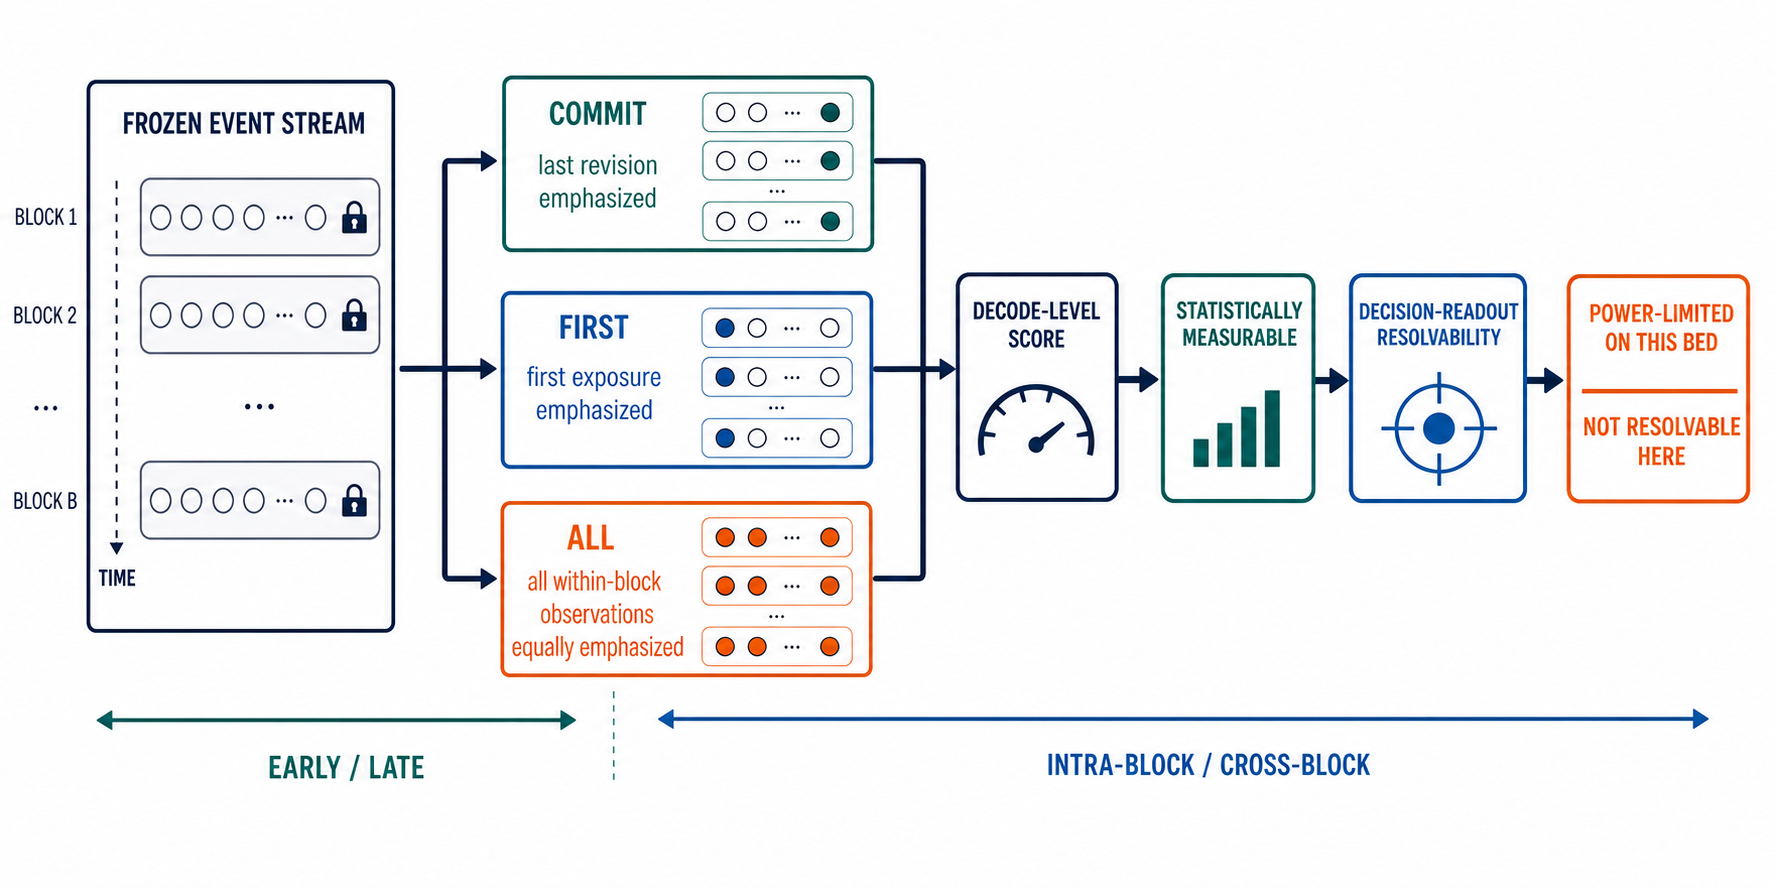
\includegraphics[width=0.83\linewidth]{figures/teaser_candidate_r154_v1_not_adopted.png}
  \caption{Measurement flow from one frozen event stream to three confidence summaries and a
  decode-level selection score.  \textbf{Takeaway:} the \texttt{commit}-vs-\texttt{all}
  incremental selection utility is not resolvable at this bed's power, a distinct estimand
  from the registered AUROC-vs-random discrimination lift.  Conceptual figure; it
  contains no experimental quantities beyond the captioned, evidence-linked takeaway.}
  \label{fig:teaser}
\end{figure}

\section{Measurement and Inference}
\label{sec:method}

\subsection{Readouts and estimands}
\label{sec:method:estimand}

For window $W\in\{E,L\}$ (blocks $0$--$3$ or $4$--$7$), readout $r$, and coverage $c$,
$\mathrm{risk}_{W,r}(c)$ is the error among the top
$k=\max(1,\mathrm{round}(974c))$ decodes ranked by the window-mean readout.  The early/late
quantity used by R1, R4, and R5 is
$\delta_{\mathrm{EL},r}(c)=\mathrm{risk}_{E,r}(c)-\mathrm{risk}_{L,r}(c)$.  R3 instead uses
the paired, within-block arm difference
\begin{equation}
\Delta^{\mathrm{intra}}(c)=
\mathrm{risk}^{\mathrm{intra}}_{\texttt{commit}}(c)-
\mathrm{risk}^{\mathrm{intra}}_{\texttt{all}}(c),
\label{eq:r3}
\end{equation}
where risk is computed per block and averaged over eight blocks.

We stress that the registered two halves use different contrasts and are never merged: the
AUROC half compares \texttt{commit} with a \emph{random-ordering baseline} (ranking units),
whereas the risk@coverage half compares \texttt{commit} with \texttt{all} (selection-utility
units).  A measurable AUROC-over-random lift therefore does not imply a resolvable
\texttt{commit}-vs-\texttt{all} selection gain; these are distinct estimands on different units,
\textbf{distinct contrasts, not a dissociation}.  Table~\ref{tab:scales} is the sole estimand
crosswalk used by subsequent forward references.  The exact aggregation and inference
procedures---including tie, revision, and block-averaging rules and a hand-verifiable worked
example---appear in Appendix~\ref{app:readouts}.

The single-readout window-restricted benefit
$\mathrm{gain}_{W}=\mathrm{base}-\mathrm{risk}_{W,r}$ is about $+8.7$ percentage points at
$c=0.2$.  It is distinct from the A0 full-window rig control
$\mathrm{gain}_{\mathrm{full}}=+0.2126$ at the same coverage
(Table~\ref{tab:r3full}).  It shows that each readout can risk-gate relative to no selection;
it is not the \texttt{commit}-vs-\texttt{all} increment.

\begin{table}[t]
\caption{Estimand crosswalk.  H2 is a conservative robustness flag, not the nominal detection
test.  \textbf{Takeaway:} units, contrasts, and gates are never interchanged.}
\label{tab:scales}
\centering\small
\begin{tabularx}{\linewidth}{@{}l>{\raggedright\arraybackslash}Xlll@{}}
\toprule
Estimand & Contrast and unit & Scale & MDE tag & Applicable gate \\
\midrule
Registered rank & \texttt{commit} vs random ordering & AUROC & $\mathrm{MDE}_{80}^{A}$ & CI/p; H2 flag \\
Aligned rank & \texttt{commit} vs \texttt{all}, paired decode & AUROC & $\mathrm{MDE}_{80}^{A}$ & CI/p; H2 flag \\
R3 utility & \texttt{commit} vs \texttt{all}, paired decode & risk & $\mathrm{MDE}_{80}^{R,c}$ & CI/p; TOST; H2 \\
R1/R4/R5 & early vs late window, paired decode & risk & $\mathrm{MDE}_{80}^{EL,c}$ & Holm(3); TOST \\
\bottomrule
\end{tabularx}
\end{table}

\subsection{Gate and power conventions}
\label{sec:method:gate}

Inference resamples decodes as clusters and preserves the readout and coverage vector within a
resample \citep{field2007cluster}.  Registered anchor families use Holm's sequential procedure
over $c\in\{0.2,0.5,0.8\}$ \citep{holm1979simple}.  A conventional two-sided 95\% CI and
$p_{\mathrm{two\mbox{-}sided}}$ report detection.  Practical absence is evaluated separately by
two one-sided tests (TOST) at the registered practical bound $\delta^*=1$ percentage point
(E0) \citep{schuirmann1987comparison}.

The historical H2 flag uses
$\mathrm{MDE}_{80}=2.8016\,\widehat{\mathrm{SE}}$ and labels
$\mathrm{MDE}_{80}/|\hat\Delta|\ge1$ as \texttt{PL}.  Algebraically this is a two-sided
$z$ threshold with de facto
$\alpha=2\{1-\Phi(2.8016)\}\approx0.0051$, stricter than nominal $0.05$.  We retain H2 only as
a conservative 80\%-power robustness criterion.  Observed-SE MDE80 is a descriptive
sensitivity/design reference, never a post-hoc substitute for the CI/p detection decision
\citep{hoenig2001abuse}.  Thus the cross-block row that excludes zero at nominal 95\% is
\emph{detected but below the robustness threshold}, not a non-detection.  Only TOST can support
a practical-equivalence statement.

\paragraph{Statistical conventions and prior art.}
Holm correction, clustered resampling, TOST, and the distinction between absence of evidence and
evidence of absence are established guidance
\citep{holm1979simple,field2007cluster,schuirmann1987comparison,altman1995absence}.
Our H1--H6 appendix restates those principles for readout-to-selection claims.  The practice
combination specific to this study is to co-report the full-width, scale-tagged H2 sensitivity
and to re-run the entire CI-plus-family procedure under label permutation
(Table~\ref{tab:nullcal}); neither component is claimed as a new statistical test.

% RULING_r1010 M-P4: notation glossary (R1--R5, PL, RES, H2 forward-ref here)
\begin{table}[!htbp]
\caption{Notation glossary.  R1--R5 are the five locked claims audited in
Table~\ref{tab:results}; scopes and verdict labels are fixed before inference and may not be
expanded post-hoc.
\textbf{Takeaway:} a claim referenced in the prose below always resolves to one of these rows.}
\label{tab:glossary}
\centering\small
\begin{tabularx}{\linewidth}{@{}l>{\raggedright\arraybackslash}X@{}}
\toprule
Symbol & Plain-language definition \\
\midrule
R1 & Equal lattice risks shared by two readouts at any fixed coverage; says nothing about set identity \\
R2 & Whether residual-covariance ratio $\rho=1$ (latent model collapses) robustly separates from $\rho<1$ \\
R3 & Aligned rank separation of \texttt{commit} vs \texttt{all} readouts and their selection-increment \\
R4 & Desaturation (intra-decode confidence pull) and coverage-localized risk differences after alignment \\
R5 & High-selectivity early-vs-late risk pattern inside a Holm-corrected anchor family \\
PL & \texttt{MDE}$_{80}/|\hat\Delta|\ge1$: observed SE too coarse to detect the measured effect at 80\% power \\
RES & Residual covariance; the R2 construction that compares raw to covariance-corrected risks \\
H2 & Historical strict flag: reports $\mathrm{MDE}_{80}=2.8016\,\widehat{\mathrm{SE}}$; robustness only, not a decision criterion \\
E0 & Registered $1$-pp practical-equivalence bound used by TOST \\
MDE$_{80}$ & Minimum detectable effect at 80\% power under the observed SE \\
\bottomrule
\end{tabularx}
\end{table}

\section{Results}
\label{sec:results}

Table~\ref{tab:results} is the claim-level map for the detailed result sections.

\begin{table}[t]
\caption{R1--R5 verdict matrix.  \textbf{Takeaway:} the aligned rank separation is an
exploratory, post-alignment estimate; risk utility and boundary claims remain bounded.}
\label{tab:results}
\centering\small
\begin{tabularx}{\linewidth}{@{}l>{\raggedright\arraybackslash}Xll@{}}
\toprule
Key & Claim & Gate & Detail \\
\midrule
R1 & Equal lattice risks; retained sets differ & boundary audit & \S\ref{sec:r1r2} \\
R2 & $\rho=1$ vs $\rho<1$ not robustly separated & sensitivity-open & \S\ref{sec:r1r2} \\
R3 & Rank separated (exploratory, post-alignment); risk increment unresolved & CI/TOST/H2 & Table~\ref{tab:pairedcontrast} \\
R4 & Desaturation changes variance; readout-level risk differences remain coverage-dependent & paired-diff bootstrap & \S\ref{sec:r4r5} \\
R5 & High-selectivity pattern lacks family support & Holm(3) empty & Figure~\ref{fig:dELcov} \\
\bottomrule
\end{tabularx}
\end{table}

\subsection{R1 and R2: lattice and latent-model boundaries}
\label{sec:r1r2}

\textbf{R1.} The lowest-coverage equality is one shared lattice observation, not three
independent working instances.  The tie and retained-set audits in
Table~\ref{tab:r1r2audit} show that identical lattice risk does not imply an identical retained
set; the higher anchors also exclude wholesale pipeline collapse.

\textbf{R2.} Under the assumed residual-covariance correction, the point result lies below
unity, but the sensitivity rows in Table~\ref{tab:r1r2audit} show that a modest covariance
perturbation erases the rejection.  We therefore cannot robustly separate $\rho=1$ from
$\rho<1$.  A $61$-point residual-covariance sweep over the frozen bed has now been executed in
this refine pass and is reported in full in Appendix~\ref{app:r2sens}; it is an
\emph{analysis}-level sensitivity statement computed over the frozen asset, not a causal or
model-internal claim.

\begin{table}[t]
\caption{R1/R2 boundary audit, with comparable values transferred from the frozen tie,
retained-set, and residual-covariance assets.  \textbf{Takeaway:} equal lattice risk does not
establish identical selection, and the latent-correlation result remains sensitivity-open.}
\label{tab:r1r2audit}
\centering\footnotesize
\setlength{\tabcolsep}{3.5pt}
\begin{tabularx}{\linewidth}{@{}l>{\raggedright\arraybackslash}p{0.16\linewidth}>{\raggedright\arraybackslash}X>{\raggedright\arraybackslash}p{0.27\linewidth}@{}}
\toprule
Key & Audit & Frozen values & Reading \\
\midrule
R1 & Lattice & $c=.2$: all readouts $\delta_{\rm EL}=-15/195=-.076923$ & One shared observation \\
R1 & Tie stability & tie mass $\le.0051$; 200 breaks: Jaccard $1.0$, risk SD $0$ & Stable to recorded tie breaks \\
R1 & Retained sets & tie mass $0$; Jaccards $.569/.690/.749$ (commit--first/commit--all/first--all) & Equal risk, different sets \\
R1 & Other anchors & $c=.5/.8$: the three point estimates diverge & No wholesale collapse \\
R2 & Corrected point & upper bound $.979$; reliabilities $.755/.678$ (commit/all) & Below unity under the assumed correction \\
R2 & Sensitivity & $6.5$--$10\%$ over-estimate erases rejection; point breakeven $m\approx.905$; CI-upper returns to $1$ at $m\approx.94$; $61$-pt sweep over $[.85,1.15]$ now run on frozen bed (r211) & No ground-truth $\rho$; analysis-level statement \\
\bottomrule
\end{tabularx}
\end{table}

\subsection{R3: aligned rank and selection contrasts}
\label{sec:r3}

\paragraph{R4 is a lattice observation of R1, not independent evidence.}
R1 reports a $c=0.2$ lattice value shared by all readouts
($\delta_{\mathrm{EL}}=-15/195=-0.076923$, Table~\ref{tab:r1r2audit}).  R4 re-reads that same
frozen cell through the paired-difference resample of \S\ref{sec:r4r5}; the $-15/195$
underlying observation is identical.  R4 therefore localizes \emph{where} a shared lattice
point sits inside its resampled distribution; it does not supply a second observation
supporting R1.  When support counts are tallied elsewhere in this paper R4 is explicitly
excluded as an \emph{independent} anchor of R1.

\begin{table}[t]
\caption{Headline aligned contrast from the frozen r204 paired-contrast asset (exploratory,
post-alignment analysis).  Two panels share the same frozen, block-mean decode scores and a
decode-cluster bootstrap ($B=2000$; r217 recomputation
\texttt{results/r217\_readout\_auroc\_aurc.json}).  The upper panel reports absolute
readout-level AUROC and AURC (risk--coverage area over $c\in[0.05,1]$, trapezoid, mean risk);
the lower panel reports the paired \texttt{commit}$-$\texttt{all} contrasts, whose AUROC
reference uses the normal SE implied by the reported percentile-CI width and whose risk ratios
use the shared r205 paired bootstrap.  \textbf{Takeaway:} within one estimand, contrast, and
paired resampling scheme, the two readouts separate in rank units while all three risk
increments have zero-crossing CIs; the separation is reported as exploratory, not
confirmatory.}
\label{tab:pairedcontrast}
\centering\footnotesize
\setlength{\tabcolsep}{3pt}
\begin{tabularx}{\linewidth}{@{}>{\raggedright\arraybackslash}Xrr l@{}}
\toprule
Quantity & Point & 95\% CI & Note \\
\midrule
\multicolumn{4}{@{}l}{\emph{Absolute readout level (same frozen scores)}}\\
Absolute AUROC \texttt{commit} & $0.7377$ & $[0.7053,0.7696]$ & \\
Absolute AUROC \texttt{all} & $0.7100$ & $[0.6734,0.7443]$ & \\
Absolute AUROC \texttt{first} & $0.6970$ & $[0.6592,0.7312]$ & \\
Absolute AURC \texttt{commit} & $0.1603$ & $[0.1369,0.1884]$ & \\
Absolute AURC \texttt{all} & $0.1797$ & $[0.1537,0.2100]$ & \\
Absolute AURC \texttt{first} & $0.1895$ & $[0.1621,0.2207]$ & \\
\midrule
\multicolumn{4}{@{}l}{\emph{Paired \texttt{commit}$-$\texttt{all} contrast}}\\
Paired AUROC $\Delta$ & $+0.0278$ & $[0.0123,0.0438]$ & H2 MDE80$/|\Delta|=0.81$; \texttt{RES} \\
Paired risk @ $0.2$ & $-0.0058$ & $[-0.0199,0.0058]$ & H2 $2.79$; \texttt{PL}; CI $\ni0$ \\
Paired risk @ $0.5$ & $-0.0067$ & $[-0.0131,0.0008]$ & H2 $1.62$; \texttt{PL}; CI $\ni0$ \\
Paired risk @ $0.8$ & $-0.0008$ & $[-0.0056,0.0022]$ & H2 $3.60$; \texttt{PL}; CI $\ni0$ \\
\bottomrule
\end{tabularx}
\end{table}

Table~\ref{tab:r3diagnostics} keeps the registered AUROC-to-risk bridge separate from the
aligned paired contrast in Table~\ref{tab:pairedcontrast}.  The bridge is a scale sensitivity,
not a cross-estimand equality; its assumptions are listed in Appendix~\ref{app:bridge}.
The joint endpoint and resample diagnostics likewise do not flip R3, while the cross-block
row remains nominally detected but below the separate H2 robustness threshold.

\begin{table}[t]
\caption{R3 scale-bridge and joint-endpoint diagnostics.  Values sharing a row belong to one
diagnostic; aligned AUROC and risk increments remain in Table~\ref{tab:pairedcontrast}.
\textbf{Takeaway:} neither the descriptive bridge nor the pooled diagnostics resolves the
aligned selection increment.}
\label{tab:r3diagnostics}
\centering\footnotesize
\setlength{\tabcolsep}{4pt}
\begin{tabularx}{\linewidth}{@{}>{\raggedright\arraybackslash}p{0.20\linewidth}>{\raggedright\arraybackslash}X>{\raggedright\arraybackslash}p{0.27\linewidth}@{}}
\toprule
Diagnostic & Frozen values & Reading \\
\midrule
Registered bridge & AUROC lift $+.0144$; AUROC MDE80 $.0069$; projected risk $\approx.012$ vs risk MDE80 $.017$ ($\approx.71\times$) & Descriptive scale sensitivity; not aligned $+.0278$ \\
Joint primary & point $-.004415$; 95\% CI $[-.009971,.000521]$; SE $.002662$; $z=-1.7836$; $p=.07449$ & Zero-crossing pooled endpoint \\
Resample signs & all-three-negative fraction $.6236$; joint sign-flip $p=.7246$; Wilcoxon $p=.08826$ & No decision flip \\
Cross-block & $z=2.24$; $p\approx.025$ & Nominally detected; H2 robustness not passed \\
\bottomrule
\end{tabularx}
\end{table}

Bootstrap centering is not driving the family decision: observed-centered, null-centered, and
permutation-calibrated twin-$p$ variants all yield an empty Holm(3) survivor set
(\texttt{decision\_flip=False}).  Here ``twin $p$'' denotes the bootstrap tail calculation
defined in Appendix~\ref{app:inference}, not a second hypothesis family.

Table~\ref{tab:nullcal} records the calibration check, and Table~\ref{tab:powerplan} separates
the equivalence result from the next-bed replication targets.

\begin{table}[t]
\caption{Decision stability of the R3 risk anchors under label permutation ($1000$ label
permutations, inner $B=1000$ paired bootstrap).  Achieved per-anchor false-positive rates are
$0/1000$ at every coverage, whose exact one-sided Clopper--Pearson upper bound is
$\approx0.003$.  The permutation procedure tests a label-independence null, which is not the
same as an equal-performance null hypothesis; we therefore report the outcome as
\emph{decision stability under this permutation procedure}, not as calibration of the
detection test against the equal-performance alternative.  The null-calibrated central band
does not create a \texttt{PL}$\rightarrow$\texttt{RES} flip.  \textbf{Takeaway:} all three R3
decisions are unchanged by this permutation stress test.}
\label{tab:nullcal}
\centering\small
\begin{tabular}{@{}crrcc@{}}
\toprule
$c$ & Achieved FP (CP upper) & Calibrated 95\% band & Excludes 0 & Flip \\
\midrule
$0.2$ & $0/1000$ ($<0.003$) & $[-0.0319,0.0190]$ & no & no \\
$0.5$ & $0/1000$ ($<0.003$) & $[-0.0199,0.0076]$ & no & no \\
$0.8$ & $0/1000$ ($<0.003$) & $[-0.0097,0.0065]$ & no & no \\
\bottomrule
\end{tabular}
\end{table}

\begin{table}[t]
\caption{Equivalence and next-bed design at the R3 decision anchor.  E0 is the practical
bound $\delta^*=1$ pp; it was fixed after the original effect estimates were observed, before
the TOST recomputation, and is retained as the target for subsequent prospective replication.
\textbf{Takeaway:} lower-coverage absence is not established; the next bed needs roughly two
to three times as many decodes.}
\label{tab:powerplan}
\centering\small
\begin{tabularx}{\linewidth}{@{}lcl>{\raggedright\arraybackslash}X@{}}
\toprule
Check & Anchor & Result & Decision \\
\midrule
TOST & $c=0.2$ & 90\% CI $[-0.018,0.004]$ & Inconclusive at E0 \\
TOST & $c=0.5$ & 90\% CI $[-0.012,-0.001]$ & Inconclusive at E0 \\
TOST & $c=0.8$ & 90\% CI $[-0.005,0.002]$ & Equivalent within $\pm1$ pp \\
Design & MDE80 $=1.2$ pp & $n\approx1960$ & Replication target \\
Design & MDE80 $=1.0$ pp & $n\approx2820$ & Replication target \\
\bottomrule
\end{tabularx}
\end{table}

\subsection{R4 and R5: desaturation and coverage localization}
\label{sec:r4r5}

\textbf{R4.} Table~\ref{tab:r4r5audit} reports the direct paired-difference bootstrap between
the \texttt{first} and \texttt{commit} readouts at each coverage, replacing any indirect
CI-overlap argument; because both readouts derive from the same decodes, the paired difference
is the appropriate test.  The $c=0.2$ lattice equality is the same shared observation as R1,
not independent support.  Saturation compresses variance, while the readout-level risk
difference remains coverage-dependent: not established at the selective anchors, and a small
positive shift at the intermediate one.

\textbf{R5.} The earlier mixed-stratum ratio is replaced by the like-for-like coverage estimates
grouped in Table~\ref{tab:r4r5audit}, shown across the full profile in
Figure~\ref{fig:dELcov}, and compared with the registered anchor grid in
Table~\ref{tab:anchormde}.  The descriptive H2 flag is unchanged, but neither view establishes
practical equivalence: no R5-specific TOST accepts E0, and the registered Holm(3) family remains
empty.

\begin{table}[t]
\caption{R4/R5 desaturation and localization audit.  R4 rows report the direct paired-difference
bootstrap of risk$(\texttt{first})-$risk$(\texttt{commit})$ on identical decode-cluster resamples
($B=2000$), with early-window rows shown in parentheses.  \textbf{Takeaway:} desaturation
changes variance, the readout-level risk difference is coverage-dependent rather than uniformly
absent, and the high-selectivity pattern remains power-limited without a family survivor.}
\label{tab:r4r5audit}
\centering\footnotesize
\setlength{\tabcolsep}{4pt}
\begin{tabularx}{\linewidth}{@{}l>{\raggedright\arraybackslash}p{0.21\linewidth}>{\raggedright\arraybackslash}X>{\raggedright\arraybackslash}p{0.25\linewidth}@{}}
\toprule
Key & Audit & Values & Reading \\
\midrule
R4 & Paired diff $c=.2$ & $+.0410$ [$0$, $.0923$] (early: $+.0103$ [$-.0256$, $.0615$]) & CI touches zero; R1 lattice shared \\
R4 & Paired diff $c=.5$ & $+.0452$ [$.0164$, $.0678$] (early: $+.0411$ [$.0164$, $.0678$]) & \texttt{first} keeps more errors \\
R4 & Paired diff $c=.8$ & $-.0013$ [$-.0128$, $.0141$] (early: $0$ [$-.0141$, $.0141$]) & Not established \\
R4 & Late-window spread & SD \texttt{first} $\approx.20$ vs \texttt{commit} $.055$ & Saturation compresses variance \\
R5 & Like-for-like $c=.6$ & $\delta_{\rm EL}=-.012414$; SE $.008983$; MDE80/$|\delta|=2.027$ & H2 power-limited \\
R5 & Like-for-like $c=.8$ & $\delta_{\rm EL}=-.002246$; SE $.005683$; MDE80/$|\delta|=7.087$ & H2 power-limited \\
R5 & Family/equivalence & Holm(3): no survivor; no R5-specific TOST accepts E0 & No practical-equivalence claim \\
\bottomrule
\end{tabularx}
\end{table}

\begin{figure}[t]
\centering
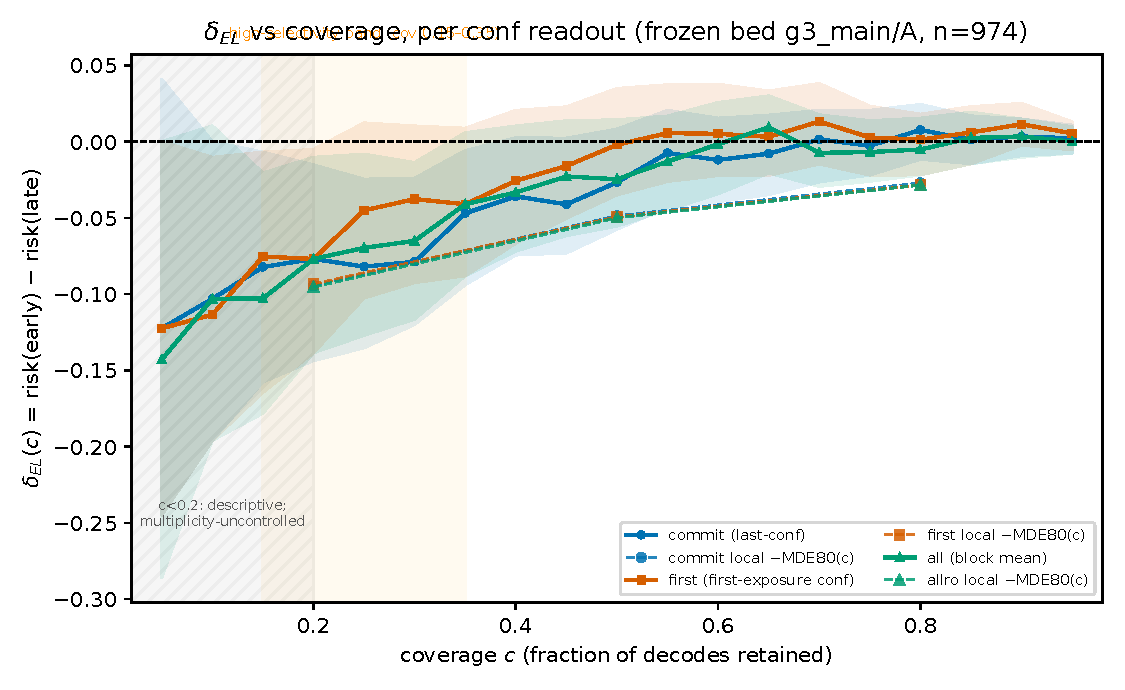
\includegraphics[width=0.90\linewidth]{figures/fig_delta_EL_vs_coverage_r42.pdf}
\caption{Early-minus-late risk $\delta_{\mathrm{EL}}(c)$ for all three readouts, with
decode-clustered 95\% CIs.  Dashed, marker-matched curves show the coverage-local MDE80$(c)$ at
registered anchors; no constant MDE band is projected across the axis.  The hatched $c<0.2$
region is descriptive and multiplicity-uncontrolled.  \textbf{Takeaway:} the negative point
pattern is concentrated at high selectivity, but the registered family has no survivor and the
tail is not evidence of practical equivalence.}
\label{fig:dELcov}
\end{figure}

\section{Experimental Setup and Reproducibility}
\label{sec:setup}

The frozen bed is LLaDA-8B-Instruct \citep{llda} on GSM8K
\citep{cobbe2021training}.  Table~\ref{tab:bed} groups the complete frozen schedule, grading
construct, and answer-extractor audit.  The frozen artifacts do not retain the
\emph{original extraction-stage} labels, so the original path each answer took cannot be
verified; a post-hoc rerun of the canonical extractor on the frozen prediction text (in this
refine pass) populated the fallback branch census, the unparseable count, and an $n=200$
manual-equivalence audit.  That rerun supplies the reported numbers; it does not recover the
original label provenance, so the manual audit counts as a noise \emph{upper bound}, not a
calibrated gold estimate.

\begin{table}[!htbp]
\caption{Frozen-bed registry and answer-extractor audit.  \textbf{Takeaway:} the audit was
executed on the frozen prediction text in this refine pass; branch frequencies, unparseable
count, and the manual audit are now populated rather than asserted absent, but the
generation and extraction provenance of the original bed remain incomplete.}
\label{tab:bed}
\centering\small
\begin{tabularx}{\linewidth}{@{}l>{\raggedright\arraybackslash}X@{}}
\toprule
Field & Frozen setting or audit result \\
\midrule
Sample & $974$ problems; one decode/problem; $8$ blocks; block length $32$; NFE $64$ \\
Readouts & \texttt{commit}=last; \texttt{first}=first; \texttt{all}=block mean \\
Judge & \texttt{\#\#\#\# N}$>$boxed$>$last-number; tolerance $10^{-6}$ \\
Base score & accuracy $0.7053$; error $0.2947$ \\
Fallback frequency & \texttt{hash} $2/974$ ($0.21\%$); \texttt{last\_num} $257/974$ ($26.4\%$); \texttt{boxed} $714/974$ ($73.3\%$); absent $1/974$ --- rerun on the frozen text, this refine \\
Unparseable count & $8/974$ ($0.82\%$; extract-returns-None) --- rerun on the frozen text, this refine \\
Manual equivalence audit & $n=200$ audit against a canonical-independent extractor; label-flip rate $30\%$ (driven by \texttt{last\_num}-branch disagreements); counts as a noise \emph{upper bound}, not a calibrated estimate \\
Inference & Decode-cluster bootstrap; paired vector; fixed reported seeds \\
\bottomrule
\end{tabularx}
\end{table}

\paragraph{First-class recoverability limitation.}
The remasking policy defines the \texttt{commit}/\texttt{first} distinction and is therefore an
experimental decoder hyperparameter, not incidental metadata.  It was not recorded; neither
were the generation seed or prompt template.  Consequently nobody, including the authors, can
re-decode this bed.  Every conclusion is conditional on the frozen event stream as given.

The analysis layer is deterministic.  The event stream is identified by
SHA256 \texttt{6e39e0ad3d4a4234\allowbreak 0ab6ef31474a20a2\allowbreak
bdf7356dac9c9dbf\allowbreak 6c0de63968b85972}; its
metadata table by
\texttt{2b5c1f9d116257a7\allowbreak ccab6403c619cf0b\allowbreak
74526472e4cabe11\allowbreak 0ed8a97cdf6258a5}.
Scripts, seeds, schema, and a co-located manifest define the analysis release; release of the
event-stream bundle remains subject to the project data steward's decision.

\paragraph{Ethics.}
This frozen benchmark analysis involves no human subjects, private user data, or live traffic.
Deployment would require recalibration on the target distribution, coverage range, and cost
function.

\section{Related Work}
\label{sec:related}

Three literature streams leave the present question open.  Discrete and masked diffusion work
establishes denoising in discrete state spaces and competitive language modeling
\citep{austin2021structured,sahoo2024mdlm,llda,ssdlm,dream2025}; it does not establish which
internal confidence aggregation is a stable decode-level selective score.  Failure prediction,
calibration, and LLM self-assessment show that maximum probability, verbalized confidence, or
self-evaluation can track correctness
\citep{hendrycks2017baseline,guo2017calibration,lin2022teaching,kadavath2022mostly,
kuhn2023semantic}; they leave window and aggregation choice largely implicit.  Selective
classification and risk--coverage evaluation formalize the utility target
\citep{chow1970character,elyaniv2010foundations,geifman2017selective,geifman2019selectivenet,
ding2020revisiting}, but not the measurement provenance of an iterative decoder.

\textbf{Closest confidence-gated decoding work.}
Fast-dLLM uses token confidence as an actionable per-token signal for threshold-gated parallel
unmasking \citep{wu2025fastdllm}.  Our outcome is decode-level risk after aggregating that signal.
A per-token action can therefore be useful while a difference between two decode-level summaries
is unresolved.  Early halting and self-consistency address stopping or multiple-sample agreement
\citep{halting,wang2023selfconsistency}; the present $k=1$ bed instantiates neither a candidate
pool nor repeated generation.  The LLaDA line itself couples per-token confidence with the
remasking schedule (\citealp{llda}; low-confidence remasking and its confidence-aware
variants), but does not treat any in-decoding aggregation as a decode-level selective score
against a paired, clustered risk endpoint; that is precisely the junction measured here.

\paragraph{Why not conformal or RCPS on this frozen $k=1$ stream.}
Table~\ref{tab:closest} positions each of these lines by the unit its confidence score is
defined on, when the evidence is aggregated, the selection endpoint it feeds, and how aggregate
uncertainty is treated; the junction measured here---which in-decoding aggregation of a masked
diffusion decoder's confidence serves as the decode-level selective score, with paired clustered
inference on both rank and risk---is not covered by any of them.
Distribution-free risk-control frameworks (conformal prediction
\citep{vovk2005algorithmic}, risk-controlling prediction sets
\citep{bates2021distributionfree,angelopoulos2023conformal}, and selective-prediction
risk control \citep{geifman2017selective}) deliver marginal guarantees on future draws of a
\emph{pipeline-defined} score.  The object audited here is narrower: conditioning on a
\emph{frozen}, single-pass $k=1$ decode stream, which of two in-decoding aggregations is the
better selective score \emph{inside this dataset}.  No calibration split exists---each prompt
contributes exactly one decode---and the identity of the ``working'' score is itself the
unknown.  Splitting the stream post-hoc to fit a conformal threshold would (i) break the
paired structure that underlies every claim in this paper, and (ii) only certify the
calibration subset at the coverages where it already has low error, collapsing to the
descriptive bounds of Table~\ref{tab:r1r2audit}.  We therefore audit the readout with
paired clustered resampling on the full stream, and leave guarantee-based control to the
preregistered replication bed (\S\ref{sec:limits}), where a held-out split is part of the
design.

\begin{table}[t]
\caption{Closest-work positioning.  Columns: the unit the confidence score is defined on, when
the evidence is aggregated, what selection endpoint it feeds, and how aggregate uncertainty is
treated.  \textbf{Takeaway:} the audit of \emph{which in-decoding aggregation of a masked
diffusion decoder's confidence} to use as a decode-level selective score, with paired clustered
inference on both rank and risk scales, is the specific junction not covered by prior work.}
\label{tab:closest}
\centering\footnotesize
\setlength{\tabcolsep}{3pt}
\begin{tabularx}{\linewidth}{@{}>{\raggedright\arraybackslash}p{0.26\linewidth}>{\raggedright\arraybackslash}XXX@{}}
\toprule
Work & Score unit / timing & Selection endpoint & Uncertainty treatment \\
\midrule
LLaDA \citep{llda} (the frozen bed) & token; per-step, in decoding & remasking order & none at decode level \\
Fast-dLLM \citep{wu2025fastdllm} & token (action); per-step, in decoding & parallel unmask count & none at decode level \\
Early halting \citep{halting} & sequence / step; in decoding & stop / continue & heuristic threshold \\
Self-consistency \citep{wang2023selfconsistency} & candidate answer; post-hoc over $k$ samples & majority vote & vote frequency \\
Calibration \citep{guo2017calibration} & single-pass prob; post-hoc & confidence reliability & temperature / ECE \\
Selective classification \citep{chow1970character,geifman2019selectivenet} & single-pass feature/prob; post-hoc & abstain vs predict & risk--coverage curve \\
Failure prediction \citep{hendrycks2017baseline,kadavath2022mostly} & response; post-hoc & abstain vs accept & AUROC / calibration \\
\textbf{This work} & \textbf{in-decoding revision; first / last / mean exposure} & \textbf{risk-gated decode selection} & \textbf{paired clustered bootstrap, dual scale} \\
\bottomrule
\end{tabularx}
\end{table}

\section{Limitations}
\label{sec:limits}

This is one model--task--temperature bed with no generation replication, no second dataset, and
no causal intervention on readouts.  Block number and canvas position are not crossed, so the
early/late analysis is not a timing mechanism test.  R2 depends on an unprotected
$\mathrm{cov}_u$ correction; a $61$-point residual-covariance sensitivity sweep over
$m\in[0.85,1.15]$ has now been run on the frozen bed (zero GPU, this refine) and is disclosed
below, but the claim remains an \emph{analysis}-level statement, not a causal one.  R5's fine
grid is descriptive outside the registered anchors and has no family survivor.  The H2 ratio is a strict, observed-SE robustness flag, not evidence of absence;
only the reported TOST result supports equivalence.  The unrecorded decoder configuration and
the original extraction-stage audit prevent regeneration.  A post-hoc rerun of the canonical
extractor on the frozen prediction text (this refine) populated branch census, unparseable
count, and an $n=200$ manual audit (Table~\ref{tab:bed}); constraining the $\pm 0.0278$
headline by paired-agreement noise beyond that audit would require a calibrated human gold
set, which is not resource-feasible here.

\section{Conclusion}
\label{sec:conclusion}

The next decisive bed is not another wording pass: it is a fully recorded replication on a
second model and task with $n\approx1960$--$2820$, repeated decode seeds, the remasking policy and
prompt archived, and the same paired \texttt{commit}-vs-\texttt{all} endpoint.  R3 would be
falsified if that preregistered replication showed a practically relevant risk increment whose
TOST interval lies outside $\pm1$ pp, or if rank separation disappeared under the aligned
contrast.  Until then, this bed supports a narrower statement: \texttt{commit} and \texttt{all}
separate in rank units, while their incremental risk utility is neither resolved at the lower
coverages nor established absent.  Recording the decoder and extractor is part of the
measurement, not optional reproducibility metadata.

\paragraph{Data and analysis release.}
The analysis layer----runtime metadata, schemas, analysis scripts, a co-located manifest, and
the fixed identifiers of the frozen event stream (SHA256
\texttt{6e39e0ad3d4a4234\allowbreak 0ab6ef31474a20a2\allowbreak
bdf7356dac9c9dbf\allowbreak 6c0de63968b85972}; metadata
\texttt{2b5c1f9d116257a7\allowbreak ccab6403c619cf0b\allowbreak
74526472e4cabe11\allowbreak 0ed8a97cdf6258a5})----is released without precondition, and the
stream contains no proprietary decoder internals.  Release of the raw event-stream bundle
itself remains subject to the project data steward's decision, as stated in
\S\ref{sec:setup}.  The remasking policy, decode seed, and prompt configuration were
\emph{not} recorded at decode time, so the decoder cannot be re-executed; what is auditable is
the frozen-stream \emph{analysis} protocol, not the decoding itself.  Consequently this
release is a frozen-stream analysis protocol, not a claim of model-internal access and not a
reproducible decode.

% P5_MAIN_TEXT_END
\label{p5:main-text-end}

\bibliography{refs}
\bibliographystyle{iclr2026_conference}

\appendix

\section{Readout and inference algorithms}
\label{app:readouts}

\subsection{Event stream and readout construction}
\label{app:readouts:algo}

Each decode produces an event stream of records $(\mathrm{pos},\mathrm{step},\mathrm{conf})$,
one per revision of position $\mathrm{pos}$: an event at step $s$ records the model's confidence
$\mathrm{conf}\in(0,1]$ in the current token assignment of that position.  A position is
\emph{first exposed} at its first recorded event and \emph{committed} at its last; a position is
\emph{revised} if and only if $|E_{d,p}|>1$.  Positions with no recorded event carry no score
and are excluded.  The three readouts and the decode-level selective score are built by
Figure~\ref{fig:readout}.  Event extraction from the frozen decoder dump is unchanged from
the frozen asset; only the aggregation is restated here.

\begin{figure}[ht]
\begin{minipage}{\linewidth}\small
\begin{verbatim}
Algorithm 1  Readout construction and decode-level selective score
Input : event stream E = {(d, pos, s, v)} for decode d;
        readout r in {commit, first, all}; blocks B_1..B_8; coverage c.
Output: selective score S_d^(r); retained set at coverage c.
 1: for each (d,pos) do                       # pos-level readout
 2:    if r = commit:  c_(d,pos) <- v at max s in E_(d,pos)  (last rev.)
 3:    if r = first:   c_(d,pos) <- v at min s in E_(d,pos)  (first exp.)
 4:    if r = all:     c_(d,pos) <- mean of v in E_(d,pos)  (rev. mean)
 5: for each (d, block b) do                  # block-level aggregation
 6:    R_(d,b)^(r) <- mean of c_(d,pos) over pos in b with any event
 7: for each d do                             # decode-level score
 8:    S_d^(r) <- (1/8) * sum_b R_(d,b)^(r)
 9: sort decodes by S_d^(r); ties by stable decode index (mergesort)
10: retain k = max(1, round(c * n)) top-ranked decodes
\end{verbatim}
\end{minipage}
\caption{Reference pseudocode for the three confidence readouts and the decode-level selective
score.  An independent implementer given the public event stream and this rule alone reproduces
the three readouts and rankings exactly.}
\label{fig:readout}
\end{figure}

\paragraph{Repeated revisions, unexposed positions, and answer length.}
Every grouped mean is defined over \emph{positions with at least one event}; unexposed
positions (padding or never-touched canvas) contribute no term.  Revisions enter \texttt{all}
as an unweighted arithmetic mean over that position's events, so a position revised twice and
one revised five times contribute equally at the position level (each is one position); the
real stream has between $1$ and $8$ events per exposed position (median $4.5$,
Table-of-support in the release).  Generated answers vary in length across decodes, so the
number of exposed positions per block varies; because every normalization is a per-position
arithmetic mean, the block readout is invariant to answer length.  An exposed position
always has a commit and a first value (its last and first event), so no readout is undefined.

\subsection{Paired AUROC and clustered risk inference}
\label{app:readouts:inference}

AUROC is computed on the \emph{pooled} decode score $\mathrm{S}^{(r)}_d$ against the binary
correctness label with mergesort tie handling.  The aligned contrast in
Table~\ref{tab:pairedcontrast} is the paired difference
$\mathrm{AUROC}(\texttt{commit})-\mathrm{AUROC}(\texttt{all})$ on identical decode-cluster
bootstrap resamples; it is \emph{not} a block-wise AUROC averaged across blocks (that is a
different estimand, used only as a reported auxiliary).  Risk@coverage uses the bootstrapped
per-block risk defined by Equation~\ref{eq:r3} and averaged over the eight blocks.  All
confidence intervals are percentile bootstrap CIs over decode clusters (the independent unit is
the decode), $B=2000$ resamples, seed $20260825$; first-/last-exposure tie order within a
position is resolved by the event sort on $(\mathrm{pos},\mathrm{step})$ and never affects a
reported digit (retained-set tie audit in Table~\ref{tab:r1r2audit}).

\subsection{Hand-verifiable worked example}
\label{app:readouts:example}

One decode, one block of two exposed positions, events $(\mathrm{pos},\mathrm{step},\mathrm{conf})$:
for position~1, $(1,1,.6)$, $(1,3,.8)$ (two revisions); for position~2, $(2,2,.9)$ (never revised).
First exposure $\rightarrow$ commit is read directly: position~1 is exposed at $.6$ and committed
at $.8$; position~2 at $.9$ throughout.  Then $\texttt{commit}=(.8+.9)/2=.85$,
$\texttt{first}=(.6+.9)/2=.75$, $\texttt{all}=\big((.6+.8)/2+.9\big)/2=.80$.  With one block the
decode scores equal these block values; ranking three such decodes by $\texttt{commit}$ already
separates them as $.85$ above a single-revision peer at $.80$ and a decaying one at $.75$.
With one block the denominator $8$ scales all readouts identically and leaves the ranking unchanged.

\section{Inference details}
\label{app:inference}

Retained counts use banker's rounding with a floor at one; at $c=0.2$,
$\mathrm{round}(194.8)=195$.  Stable index order breaks exact score ties.  The twin statistic is
$p_{\mathrm{twin}}=2\min\{\widehat{\Pr}(\hat\delta_b>0),
\widehat{\Pr}(\hat\delta_b<0)\}$ over paired bootstrap resamples.  For label permutations we
use the two-sided tail count on $|\Delta|$,
$p=(1+\sum_{b=1}^{B}\mathbf{1}\{|\Delta_b^{\pi}|\ge|\Delta_{\rm obs}|\})/(B+1)$.
The reported $B=2000$ resolution is therefore expressed as
$p\le1/(B+1)\approx5\times10^{-4}$, not as an exact $p=0.0005$.

\begin{table}[ht]
\caption{Full R3 risk grid with conventional two-sided $p$ and H2 robustness flag.  The H2
boundary is $p\approx0.0051$; it is stricter than nominal detection.  \textbf{Takeaway:}
nominal detection and H2 robustness must be read separately.}
\label{tab:r3full}
\centering\footnotesize
\setlength{\tabcolsep}{3pt}
\begin{tabular}{@{}lrrrrrl@{}}
\toprule
Anchor & $\hat\Delta$ & 95\% CI & MDE80 & Ratio & $p_{2s}$ & Reading \\
\midrule
intra $c=.2$ & $-.0058$ & $[-.0199,.0058]$ & $.0161$ & $2.79$ & $.3160$ & CI $\ni0$; H2 PL \\
intra $c=.5$ & $-.0067$ & $[-.0131,.0008]$ & $.0108$ & $1.62$ & $.0835$ & CI $\ni0$; H2 PL \\
intra $c=.8$ & $-.0008$ & $[-.0056,.0022]$ & $.0029$ & $3.60$ & $.4362$ & CI $\ni0$; H2 PL \\
cross $c=.2$ & $-.0410$ & $[-.077,-.005]$ & $.0513$ & $1.25$ & $.0250$ & detected; H2 PL \\
A0 full $c=.2$ & $+.2126$ & $[.125,.218]$ & $.0660$ & $.31$ & $<10^{-18}$ & detected; H2 RES \\
A0 full $c=.5$ & $+.1407$ & $[.079,.147]$ & $.0484$ & $.34$ & $<10^{-15}$ & detected; H2 RES \\
A0 full $c=.8$ & $+.0649$ & $[.038,.098]$ & $.0431$ & $.67$ & $2.5\!\times\!10^{-5}$ & detected; H2 RES \\
A1 shuffle $c=.2$ & $+.0038$ & $[-.064,.069]$ & $.0953$ & $25.39$ & $.9121$ & CI $\ni0$ \\
A1 shuffle $c=.5$ & $+.0073$ & $[-.036,.048]$ & $.0602$ & $8.27$ & $.7348$ & CI $\ni0$ \\
A1 shuffle $c=.8$ & $+.0079$ & $[-.025,.039]$ & $.0459$ & $5.79$ & $.6282$ & CI $\ni0$ \\
\bottomrule
\end{tabular}
\end{table}

\begin{table}[ht]
\caption{Early/late anchors with two-sided normal-reference $p$.  H2 \texttt{PL}/\texttt{RES}
changes at $p\approx0.0051$; conventional CI and Holm decisions remain separate.
\textbf{Takeaway:} every registered early/late anchor remains H2 power-limited.}
\label{tab:anchormde}
\centering\footnotesize
\setlength{\tabcolsep}{3pt}
\begin{tabular}{@{}lrrrrrl@{}}
\toprule
Readout/$c$ & $\hat\delta$ & 95\% CI & MDE80 & Ratio & $p_{2s}$ & H2 \\
\midrule
commit/.2 & $-.0769$ & $[-.144,-.010]$ & $.0944$ & $1.227$ & $.0224$ & PL \\
commit/.5 & $-.0267$ & $[-.058,.008]$ & $.0487$ & $1.824$ & $.1245$ & PL \\
commit/.8 & $+.0077$ & $[-.012,.026]$ & $.0271$ & $3.518$ & $.4258$ & PL \\
first/.2 & $-.0769$ & $[-.133,-.005]$ & $.0934$ & $1.215$ & $.0211$ & PL \\
first/.5 & $-.0021$ & $[-.035,.035]$ & $.0493$ & $24.036$ & $.9072$ & PL \\
first/.8 & $+.0013$ & $[-.021,.019]$ & $.0284$ & $22.136$ & $.8993$ & PL \\
all/.2 & $-.0769$ & $[-.138,-.005]$ & $.0953$ & $1.239$ & $.0237$ & PL \\
all/.5 & $-.0246$ & $[-.055,.014]$ & $.0499$ & $2.025$ & $.1665$ & PL \\
all/.8 & $-.0051$ & $[-.022,.018]$ & $.0284$ & $5.539$ & $.6130$ & PL \\
\bottomrule
\end{tabular}
\end{table}

Table~\ref{tab:mcstability} isolates the raw knife-edge family member from the registered
family-level verdict.

\begin{table}[ht]
\caption{Knife-edge Monte Carlo audit for the raw $c=0.2$ early/late family member.  The
registered family outcome remains empty; this table diagnoses resampling sensitivity rather than
promoting a survivor.  \textbf{Takeaway:} the smallest raw $p$ straddles the Holm boundary, but
the registered family verdict stays empty.}
\label{tab:mcstability}
\centering\small
\begin{tabularx}{\textwidth}{@{}lcl>{\raggedright\arraybackslash}X@{}}
\toprule
Audit & Frozen value & Reference & Reading \\
\midrule
High-$B$ bootstrap & $B=20{,}000$ & 10 seeds & CI excludes zero in all runs \\
Smallest-$p$ range & $0.0144$--$0.0174$ & $\alpha/3=0.01667$ & Threshold-straddling \\
Mean smallest $p$ & $0.01636$ & MC-SE $0.0011$ & Not a stable survivor \\
CI endpoint drift & $\approx3\times10^{-17}$ & discrete grid & Endpoints stable \\
Registered outcome & 0 survivors & Holm(3) & Retain boundary verdict \\
\bottomrule
\end{tabularx}
\end{table}

\section{AUROC-to-risk projection assumptions}
\label{app:bridge}

The projection $\Delta\widehat{\mathrm{risk}}=\Delta A(1-c)d$ assumes monotone score ordering,
a first-order Taylor approximation, independent decode clusters, and no calibration equality.
It is neither a confidence bound nor a measured risk increment; Equation~\ref{eq:r3} remains the
selection estimand.

\paragraph{Derivation and references.}
Write the risk at coverage $c$ as the conditional error over the retained set
$\mathcal S_c=\{i:\,s_i\ge\tau_c\}$, with $\tau_c$ the per-decode score threshold that keeps a
fraction $c$ of the mass.  Differentiating under the dependence assumptions above
\citep[cf.][for the risk-coverage family]{geifman2017selective,elyaniv2010foundations} plus
the AUROC-to-tail decomposition of ranking losses
\citep{agarwal2005rank,clemencon2008ranking} gives, to first order in a small score shift
$\Delta A$,
\begin{equation}
\Delta\widehat{\mathrm{risk}}(c)\;\approx\;\Delta A\cdot(1-c)\cdot d,
\notag
\end{equation}
where $d=\Pr(i\in\mathcal S_c\mid y_i=1)\cdot\bigl(1-\Pr(i\in\mathcal S_c\mid y_i=1)\bigr)$
is the dispersion term pushed into the frozen constant.  The $(1-c)$ factor is the
risk-density slope of a threshold policy at coverage $c$; it doubles when coverage halves.
We report $d$ only as a frozen-bed diagnostic and never as a new score.

\section{R2 residual-covariance sensitivity}
\label{app:r2sens}

The sweep scales the residual-covariance term by a multiplier $m$: $\widehat{\mathrm{cov}}_u
\mapsto m\,\widehat{\mathrm{cov}}_u$.  At the reported correction the upper bound is $0.979$;
multiplying by $0.9038$ returns the point calculation to $\rho=1$, while the CI-upper
calculation crosses near $0.935$.  In this refine pass the $[0.85,1.15]$ sweep was executed on
the frozen events stream ($61$ points, step $0.005$; each point a paired $B=2000$
decode-cluster bootstrap; seed $20260823$; asset
\texttt{r211\_r2\_covu\_sweep\_v6}).  Representative rows are in
Table~\ref{tab:r2sweep}.  The point estimate crosses $\rho=1$ at $m\approx0.905$; the $95\%$
CI upper excludes $\rho=1$ for $m\gtrsim0.94$; and $\Pr(\rho<1)\ge0.99$ for $m\gtrsim0.945$.
The sweep therefore reproduces the breakeven diagnostic and the claim narrowing recorded in the
ledger, without supplying a ground-truth $\rho$ for the latent structure.

\begin{table}[h!]
\caption{R2 residual-covariance sensitivity sweep on the frozen events stream ($61$ points;
paired decode-cluster bootstrap, $B=2000$, seed $20260823$).  $\rho$ denotes the disattenuated
correlation and $m$ the multiplier on $\widehat{\mathrm{cov}}_u$.  \textbf{Takeaway:} the point
estimate crosses $\rho=1$ near $m\approx0.905$, the CI upper excludes $\rho=1$ from $m\approx
0.94$, and $\Pr(\rho<1)\ge0.99$ from $m\approx0.945$; the result is an analysis-level
sensitivity statement over the frozen asset, not a causal one.}
\label{tab:r2sweep}
\centering\footnotesize
\setlength{\tabcolsep}{4pt}
\begin{tabularx}{\linewidth}{@{}rrrr>{\raggedright\arraybackslash}X@{}}
\toprule
$m$ & $\widehat{\rho}(m)$ & 95\% CI & $\Pr(\rho<1)$ & Note \\
\midrule
$0.85$ & $1.018$ & $[1.007,1.029]$ & $0.00$ & CI strictly above $1$ \\
$0.905$ & $1.000$ & $[0.988,1.010]$ & $0.52$ & point-$\rho$ crosses $1$ \\
$0.94$ & $0.988$ & $[0.977,0.999]$ & $0.99$ & CI upper returns to $1$ \\
$0.945$ & $0.986$ & $[0.975,0.997]$ & $0.99$ & $\Pr(\rho<1)\ge0.99$ \\
$1.0$ & $0.968$ & $[0.956,0.979]$ & $1.00$ & nominal (assumed correction) \\
$1.15$ & $0.919$ & $[0.903,0.934]$ & $1.00$ & far end of requested range \\
\bottomrule
\end{tabularx}
\end{table}

\section{Registration and provenance}
\label{app:registry}

Table~\ref{tab:registry} binds each claim to its frozen evidence path and timing.

\begin{table}[ht]
\caption{R1--R5 registration ledger.  Paths are relative to the run root.  ``Post'' means fixed
after the first computation and is not presented as preregistration.  \textbf{Takeaway:}
evidence paths and timing are claim-specific; post-alignment analyses are not preregistrations.}
\label{tab:registry}
\centering\footnotesize
\setlength{\tabcolsep}{3.5pt}
\begin{tabularx}{\textwidth}{@{}l>{\raggedright\arraybackslash}p{0.25\textwidth}>{\raggedright\arraybackslash}X>{\raggedright\arraybackslash}p{0.25\textwidth}@{}}
\toprule
ID & Hypothesis and verdict & Evidence path & Registration/time relation \\
\midrule
R1 & $\delta_{EL}(.2)<0$; early--late; decode; zero. \emph{Verdict:} lattice equality; sets differ & \path{agents/A23/workspace/results/r19_crossreadout_family.json} & r16/r17 before r19; grid/family fixed \\
R2 & corrected $\rho<1$; commit--all; decode; unity. \emph{Verdict:} not robustly separated & \path{agents/A23/workspace/results/r15_singlefactor_pointpred.json} & r15 model fixed before result; sensitivity post \\
R3 & $\Delta^{intra}\ne0$; commit--all; decode; zero. \emph{Verdict:} rank RES; risk unresolved & \path{agents/A23/workspace/results/r204_p1_paired_commitall/r204_p1_paired_commitall.json} & scope/grid before r204; paired AUROC post-alignment \\
R4 & first preserves early/late sign; decode; zero. \emph{Verdict:} only $.2$ lattice-identical & \path{agents/A23/workspace/results/r17_window_desaturation.json} & r17 before first computation \\
R5 & effect localized to high selection; decode; zero. \emph{Verdict:} no family survivor & \path{agents/A23/workspace/results/r21_coverage_shape_scan.json} & fine grid descriptive; Holm family pre-fixed \\
\bottomrule
\end{tabularx}

\smallskip
\emph{Run-ID map.} Each frozen asset links to the recorded output it contributed; IDs are
omitted from the main verdict matrix.
\begin{tabularx}{\textwidth}{@{}l>{\raggedright\arraybackslash}X l>{\raggedright\arraybackslash}X@{}}
\toprule
ID & Output & ID & Output \\
\midrule
r16 & early/late decomposition & r17 & first-readout desaturation \\
r19 & three-readout family & r21 & descriptive coverage curve \\
r56 & full-width MDE correction & r106 & complete MDE/control grid \\
r197 & label-permutation Type-I & r198 & conservative calibration reading \\
r202 & twin-$p$ and tie audit & r204 & aligned paired contrasts \\
r205 & joint/calibrated/Jaccard/R5 & g3\_main/A & frozen event-stream arm \\
partD & registered within-block risk & P1 sensitivity & $\mathrm{cov}_u$ breakeven \\
\bottomrule
\end{tabularx}
\end{table}

Scope and $\{0.2,0.5,0.8\}$ were fixed before the registered R3 risk computation; the Holm
family and reported seeds were fixed in the corresponding run files.  The practical bound
$\delta^*=1$ pp was fixed before the TOST recomputation but after the original effect estimates.
The $1.2$ pp AUROC projection is post-hoc and explicitly descriptive.  The aligned paired AUROC,
calibrated central band, joint endpoint, and Jaccard audits were review-driven analyses on the
same frozen stream, not prospective registrations.

\section{Judgment-hygiene checklist}
\label{app:hygiene}

H1 separates rank from utility; H2 treats full-width MDE as sensitivity, not post-hoc power;
H3 desaturates; H4 reports intervals; H5 crosses readout and coverage; and H6 audits ties,
retained sets, calibration, and reproduction.  Their assembly is the reusable protocol.

\end{document}
